%!TEX root = CooperBarba2014.tex

It is possible to derive a closed-form expression for the free energy of interaction between a spherical molecule with a centered charge and a spherical surface with imposed potential or charge, like the one sketched in Figure \ref{fig:twosphere_an}.  There are such analytical expressions for interacting charged surfaces,\cite{CarnieChanGunning1994} and interacting spherical molecules with multiple point charges inside,\cite{LotanHead-Gordon2006} but not for a situation where surfaces and molecules interact. Having such an analytical solution is of great utility in the development of a computational model for protein-surface interaction, because it will allow for proper code verification. 


\subsection{Expansion in Legendre polynomials} \label{sec:expansion_analytical}


The system of partial differential equations from Equation \eqref{eq:pde}  models the electrostatic potential field in the setting of Figure \ref{fig:twosphere_an}. Following Carnie and co-workers, \cite{CarnieChanGunning1994} the axial symmetry lets us formulate the solution of Equation \eqref{eq:pde} as an expansion in Legendre polynomials:
 

\begin{align} \label{eq:derivation1}
\phi_1 = \sum_{n=0}^{\infty} c_n r_1^n P_n(\cos \theta_1) & + \frac{q}{4\pi\epsilon_1 r_1} \quad \text{on $\Omega_1$,} \nonumber \\
\phi_2 = \sum_{n=0}^{\infty} a_n k_n(\kappa r_1) P_n (& \cos \theta_1) \nonumber \\
+ \sum_{n=0}^{\infty} b_n k_n & (\kappa r_2) P_n(\cos \theta_2) \quad \text{ on $\Omega_2$,}
\end{align}

\noindent being $P_n$ the $n^{\text{th}}$-degree Legendre polynomial and $k_n$ the modified spherical Bessel function of the second kind. 

 

\begin{figure}%[h] 
   \centering
   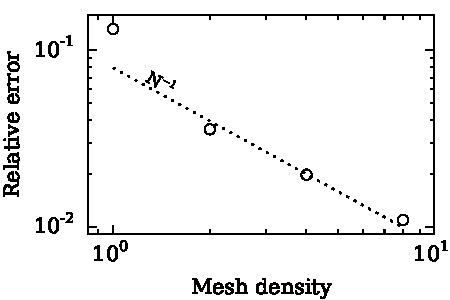
\includegraphics[width=0.45\textwidth]{Figure7.pdf} 
   \caption{Sketch of system solved with Legendre polynomials expansions.}
   \label{fig:twosphere_an}
\end{figure}
 

We make use of the following addition formula, \cite{MarceljaMitchellNinhamSculley1977}
%
\begin{equation} \label{eq:addition_formula}
k_n(\kappa r_2) P_n(\cos \theta_2) = \sum_{m=0}^{\infty}(2m+1) B_{nm} i_m(\kappa r_1) P_m(\cos \theta_1),
\end{equation}
%
\noindent to reformulate the expression for $\phi_2$ in Equation \eqref{eq:derivation1} as 
%
\begin{align} \label{eq:derivation2}
\phi_2 =& \sum_{n=0}^{\infty} a_n k_n(\kappa r_1) P_n(\cos \theta_1) \nonumber \\
& + \sum_{n=0}^{\infty} b_n \sum_{m=0}^{\infty}(2m+1) B_{nm} i_m(\kappa r_1) P_m(\cos \theta_1) \nonumber \\ 
\phi_2 =& \sum_{n=0}^{\infty} b_n k_n(\kappa r_2) P_n(\cos \theta_2) \nonumber \\
& + \sum_{n=0}^{\infty} a_n \sum_{m=0}^{\infty}(2m+1) B_{nm} i_m(\kappa r_2) P_m(\cos \theta_2).
\end{align}

Here, $i_m$ is the modified spherical Bessel function of the first kind; $B_{nm}$ is defined by 

\begin{equation} \label{eq:Bnm}
B_{nm} = \sum_{\nu=0}^{\infty} A_{nm}^{\nu} k_{n+m-2\nu}(\kappa R),
\end{equation}

\noindent where $R$ is the center-to-center distance; and $A_{nm}^{\nu}$ is given by the following expression, with ${\bf \Gamma}$ (in this context only) representing the gamma function:

%\begin{widetext}
\begin{equation} \label{eq:Anm}
A_{nm}^{\nu} = \frac{{\bf \Gamma}(n-\nu+0.5){\bf \Gamma}(m-\nu+0.5){\bf \Gamma}(\nu+0.5)(n+m-\nu)!(n+m-2\nu+0.5)}{\pi {\bf \Gamma}(m+n-\nu+1.5)(n-\nu)!(m-\nu)!\nu!}.
\end{equation}
%\end{widetext}



Legendre polynomials are orthogonal to each other, and $\frac{q}{4\pi\epsilon_1 r_1}$ is independent of $\theta$. Thus, taking the inner product of the expressions in Equations \eqref{eq:derivation1} and  \eqref{eq:derivation2} with $P_j(\cos \theta_i)$, where $i=1$ or $2$, yields
%
\begin{equation} \label{eq:derivation3}
\phi_1\delta_{0j} = c_j r_1^j + \frac{q}{4\pi\epsilon_1 r_1} \delta_{0j}  
\end{equation}
\noindent for the first expression of Equation \eqref{eq:derivation1}, and
%
\begin{align} \label{eq:derivation3.5}
\phi_2\delta_{0j} = &a_j k_j(\kappa r_1) + \sum_{n=0}^{\infty} b_n(2j+1)B_{nj} i_j(\kappa r_1),  \nonumber \\
\phi_2\delta_{0j} = &b_j k_j(\kappa r_2) + \sum_{n=0}^{\infty} a_n(2j+1)B_{nj} i_j(\kappa r_2)  
\end{align}
\noindent for Equation \eqref{eq:derivation2}.

Applying the interface conditions for $\Gamma_1$ on Equation \eqref{eq:derivation3} and the first expression of Equation \eqref{eq:derivation3.5}, produces
%
\begin{align}\label{eq:derivation4}
\sum_{n=0}^{\infty} a_n \left( \kappa k_{n}'(\kappa d_1) - \frac{\epsilon_1}{\epsilon_2} \frac{n}{d_1} k_n(\kappa d_1) \right) \delta_{nj} +& \nonumber \\ 
b_n (2j+1)B_{nj} \left( \kappa i_{j}'(\kappa d_1) - \frac{\epsilon_1}{\epsilon_2} \frac{j}{d_1} i_j(\kappa d_1)  \right) & = \nonumber \\
-\frac{\epsilon_1}{\epsilon_2} \frac{q}{4\pi\epsilon_1 d_1^2} \delta_{0j}&(j+1),
\end{align}

\noindent where $d_1$ is the radius of surface $1$.

\subsubsection*{Constant potential $\phi$ on $\Gamma_2$.}
The application of the boundary condition on $\Gamma_2$, $\phi(\Gamma_2) = \phi_0$, where $\phi_0$ is independent on $\theta_2$, gives

\begin{equation} \label{eq:derivation5_phi}
\sum_{n=0}^{\infty} a_n(2j+1)B_{nj}i_j(\kappa d_2) + b_nk_n(\kappa d_2) \delta_{nj} = \phi_0 \delta_{0j}.
\end{equation}

\noindent Combining Equations \eqref{eq:derivation4} and  \eqref{eq:derivation5_phi} yields the following system of equations for the coefficients $a_n$ and $b_n$
%
\begin{align} \label{eq:system_phi}
\mathbf{I} \mathbf{A} + \mathbf{L} \mathbf{B} &= -\frac{\epsilon_1}{\epsilon_2} \frac{q}{4\pi\epsilon_1 d_1^2} \mathbf{e} \nonumber \\
\mathbf{M} \mathbf{A} + \mathbf{I} \mathbf{B} &= \phi_0 \mathbf{e}
\end{align}

\noindent where
%
\begin{align} \label{eq:phi_terms}
I_{jn} &= \delta_{jn} \nonumber \\
e_j &= \delta_{0j} \nonumber \\
A_n &= a_n \left(\kappa k_n'(\kappa d_1) - \frac{\epsilon_1}{\epsilon_2} \frac{n}{d_1} k_n(\kappa d_1) \right) \nonumber \\
B_n &= b_n k_n(\kappa d_2) \nonumber \\
L_{jn} &= (2j+1)B_{nj}\left( \kappa \frac{i_j'(\kappa d_1)}{k_n(\kappa d_2)} - \frac{\epsilon_1}{\epsilon_2} \frac{j}{d_1} \frac{i_j(\kappa d_1)}{k_n(\kappa d_2)} \right) \nonumber \\
M_{jn} &= (2j+1)B_{nj} i_j(\kappa d_2) \frac{1}{\left(\kappa k_n'(\kappa d_1) - \frac{\epsilon_1}{\epsilon_2} \frac{n}{d_1} k_n(\kappa d_1) \right)}. 
\end{align}

\subsubsection*{Constant surface charge $\sigma$ on $\Gamma_2$.}
In this case, the application of the boundary condition on $\Gamma_2$, $\sigma(\Gamma_2) = -\epsilon_2 \frac{\partial \phi}{\partial \mathbf{n}} \Large|_{\Gamma_2} = \sigma_0$, where $\sigma_0$ is independent on $\theta_2$, gives

\begin{equation} \label{eq:derivation5_dphi}
\sum_{n=0}^{\infty} a_n(2j+1)B_{nj}\kappa i_j'(\kappa d_2) + b_n \kappa k_n'(\kappa d_2) \delta_{nj} = -\frac{\sigma_0}{\epsilon_2} \delta_{0j}
\end{equation}

\noindent Combining Equations \eqref{eq:derivation4} and  \eqref{eq:derivation5_phi} produces a system of equations for the coefficients $a_n$ and $b_n$
%
\begin{align} \label{eq:system_dphi}
\mathbf{I} \mathbf{A} + \mathbf{L} \mathbf{B} &= -\frac{\epsilon_1}{\epsilon_2} \frac{q}{4\pi\epsilon_1 d_1^2} \mathbf{e} \nonumber \\
\mathbf{M} \mathbf{A} + \mathbf{I} \mathbf{B} &= -\frac{\sigma_0}{\epsilon_2} \mathbf{e}
\end{align}

\noindent where
%
\begin{align} \label{eq:dphi_terms}
I_{jn} &= \delta_{jn} \nonumber \\
e_j &= \delta_{0j} \nonumber \\
A_n &= a_n \left(\kappa k_n'(\kappa d_1) - \frac{\epsilon_1}{\epsilon_2} \frac{n}{d_1} k_n(\kappa d_1) \right) \nonumber \\
B_n &= b_n \kappa k_n'(\kappa d_2) \nonumber \\
L_{jn} &= (2j+1)B_{nj}\left( \frac{i_j'(\kappa d_1)}{k_n'(\kappa d_2)} - \frac{\epsilon_1}{\epsilon_2} \frac{j}{d_1} \frac{i_j(\kappa d_1)}{\kappa k_n'(\kappa d_2)} \right) \nonumber \\
M_{jn} &= (2j+1)B_{nj} \kappa i_j'(\kappa d_2) \frac{1}{\left(\kappa k_n'(\kappa d_1) - \frac{\epsilon_1}{\epsilon_2} \frac{n}{d_1} k_n(\kappa d_1) \right)}. 
\end{align}
 
\subsection{Energy calculation} \label{energy_analytical}


 \medskip
 \paragraph*{Solvation free energy of the molecule---}
According to Equation \eqref{eq:solv_energy}, the solvation free energy of a molecule with a centered charge is given by
%
\begin{equation} \label{eq:energy_phi}
F_{\text{solv}} = \frac{1}{2} q \phi_{\text{reac}}(r_1=0),
\end{equation} 
 
 \noindent and using Equation \eqref{eq:derivation1}, the reaction potential from Equation \eqref{eq:phi_reac_bem} is:
 %
 \begin{equation} \label{eq:phi_reac_an}
 \phi_{\text{reac}} = \phi - \frac{q}{4\pi\epsilon_1 r} = \sum_{n=0}^{\infty} c_n r^n P_n(\cos \theta_1).
 \end{equation}
 
 Applying the boundary conditions at $\Gamma_1$ on Equation  \eqref{eq:derivation3}, we can rewrite $c_j$ in terms of the already computed $a_j$ and $b_j$:
 %
 \begin{align}
 c_j = \frac{1}{d_1^j} & \Big(a_j k_j(\kappa d_1) + \nonumber \\
&  \sum_{m=0}^{\infty} b_m(2j+1)B_{mj} i_j(\kappa d_1) - \frac{q}{4\pi\epsilon_1 d_1} \delta_{0j} \Big)
 \end{align} 
 
Because the charge is located at $r=0$, only the $n=0$ terms of Equation \eqref{eq:phi_reac_an} will survive, and the potential at this location is:
 
 \begin{align} \label{eq:phi_reac_an2}
 \phi_{\text{reac}} (r_1=0) = & a_0 k_0(\kappa d_1) + \nonumber \\
 &\sum_{m=0}^{\infty} b_m B_{m0}i_0(\kappa d_1) - \frac{q}{4\pi\epsilon_1 d_1}
 \end{align}
 
 The result from Equation \eqref{eq:phi_reac_an2} in Equation \eqref{eq:energy_phi} yields the solvation free energy. 
 
For the isolated molecule, $R \to \infty$ makes $B_{nm} \to 0$, which nullifies the sum in Equation \eqref{eq:phi_reac_an2} and $a_0$ for $R \to \infty$, from the system in Equation \eqref{eq:system_phi}, is 

\begin{equation} \label{eq:a0_inf}
a_0^{\infty} = -\frac{q}{d_1^2}\frac{\epsilon_1}{\epsilon_2} \frac{1}{4\pi\kappa k_0'(\kappa d_1) \epsilon_1}
\end{equation}


\medskip
\paragraph*{Surface  free energy with set potential $\phi_0$---}
We can expand $G_p$ from Equation \eqref{eq:energy_surf} in Legendre polynomials as
%
\begin{align} \label{eq:G_p}
G_p = &-\frac{\epsilon_2 \kappa}{\phi_0}  \Bigg[ \sum_{n=0}^{\infty} b_n k_n'(\kappa d_2) P_n(\cos \theta_2) \nonumber \\ 
& + \sum_{n=0}^{\infty} a_n \sum_{m=0}^{\infty} (2m+1) B_{nm} i_m'(\kappa d_2) P_m(\cos \theta_2) \Bigg].
\end{align}

 \noindent Applying Equation \eqref{eq:G_p} in Equation \eqref{eq:energy_surf} gives

\begin{equation} \label{G_p_int}
F = 2\pi \kappa \phi_0 d_2^2 \epsilon_2 \left[ b_0 k_0'(\kappa d_2) + \sum_{n=0}^{\infty} a_n B_{n0} i_0'(\kappa d_2) \right]
\end{equation}

 \noindent If the surface is isolated, $R \to \infty$ makes $B_{n0} \to 0$, and the free energy in this case is 
%
\begin{equation} \label{energy_isolated_phi}
F = 2\pi \kappa \phi_0 d_2^2 b_0^{\infty} k_0'(\kappa d_2) \epsilon_2
\end{equation}
 
 \noindent where $b_0^{\infty}$ is taken from the system in  \eqref{eq:system_phi} considering $B_{nm} \to 0$, which results in
 %
 \begin{equation} \label{b_inf_phi}
 b_0^{\infty} = \frac{\phi_0}{k_0(\kappa d_2)}.
 \end{equation}
 
 \medskip
 \paragraph*{Surface  free energy with set charge $\sigma_0$---}
We can expand $G_c$ from Equation \eqref{eq:energy_surf} in Legendre polynomials as
%
\begin{align} \label{eq:G_c}
G_c = & \frac{1}{\sigma_0} \Bigg[ \sum_{n=0}^{\infty} b_n k_n(\kappa d_2) P_n(\cos \theta_2) + \nonumber \\ 
&\sum_{n=0}^{\infty} a_n \sum_{m=0}^{\infty} (2m+1) B_{nm} i_m(\kappa d_2) P_m(\cos \theta_2) \Bigg]
\end{align}

 \noindent Applying Equation \eqref{eq:G_c} into Equation \eqref{eq:energy_surf} gives

\begin{equation} \label{G_c_int}
F = 2\pi \sigma_0 d_2^2 \left[ b_0 k_0(\kappa d_2) + \sum_{n=0}^{\infty} a_n B_{n0} i_0(\kappa d_2) \right]
\end{equation}

 \noindent For the isolated surface, $R \to \infty$ and $B_{n0} \to 0$, and the free energy is 
%
\begin{equation} \label{energy_isolated_dphi}
F = 2\pi \sigma_0 d_2^2 b_0^{\infty} k_0(\kappa d_2) 
\end{equation}
 
 \noindent where $b_0^{\infty}$ is calculated from the system in  \eqref{eq:system_dphi} considering $B_{nm} \to 0$, which results in
 
 \begin{equation} \label{b_inf_dphi}
 b_0^{\infty} = -\frac{\sigma_0}{\epsilon_2 \kappa k_0'(\kappa d_2)}.
 \end{equation}
